%%%%%%%%%%%%%%%%%%%%%%%%%%%%%%%%%%%%%%%%%%%%%%%%%%%%%%%%%%%%%%
% Algorithms
%%%%%%%%%%%%%%%%%%%%%%%%%%%%%%%%%%%%%%%%%%%%%%%%%%%%%%%%%%%%%%
\documentclass[../paper.tex]{subfiles}
\begin{document}
    This section provides an overview of the partitioning algorithms implemented
    in the framework, detailing their underlying principles and computational properties.
    Through illustrative examples and visual representations, we highlight the behavior of each algorithm.

%%%%%%%%%%%%%%%%%%%%%%%%%%%%%%%%%%%%%%%%%%%%%%%%%%%%%%%%%%%%%%
% Geometric-based
%%%%%%%%%%%%%%%%%%%%%%%%%%%%%%%%%%%%%%%%%%%%%%%%%%%%%%%%%%%%%%
    \subsection{Geometric-based partitioning algorithms}
    \label{subsec:geo}
    This class of bisection algorithms operates under the assumption that the geometric layout of the
    graph is known.
    These algorithms exploit spatial information of the vertices to guide the
    partitioning process, aiming to minimize edge cuts while preserving geometric
    coherence\cite{doi:10.1137/S1064827594275339}.
    This approach is particularly well suited for applications where the graph structure
    arises from physical systems, such as finite element meshes in numerical computing,
    where the underlying geometry directly influences computational efficiency\cite{buluc2015recentadvancesgraphpartitioning}. Unless stated otherwise, all function calls presented in this section take as input a graph adjacency matrix \texttt{A} and a node coordinate matrix \texttt{coords}, and return a vector assigning each node to partition 1 or 2.
%%%%%%%%%%%%%%%%%%%%%%%%%%%%%%%%%%%%%%%%%%%%%%%%%%%%%%%%%%%%%%    
    \subsubsection{Coordinate bisection}
    \label{subsubsec:coord}
    Coordinate bisection seeks a hyperplane orthogonal to one of the coordinate axes that partitions the graph's vertices into two subsets of approximately equal size
    while minimizing the edge cut.
    The algorithm computes the median $\bar{x}_j$ of each coordinate $x_j$,
    dividing all graph vertices into two groups: one containing vertices with $x_j \leq \bar{x}_j$ and the other $x_j > \bar{x}_j$. The edge cut is then evaluated for each coordinate axis, and the
    partitioning is performed along the axis that yields the smallest edge cut.
    This process in a $d$-dimensional space is summarized in \Cref{alg:coord}, with an example illustrated in \Cref{fig:coord}.
    \begin{figure}[h!]
    \centering
    \begin{subfigure}[b]{0.23\textwidth}
        \centering
        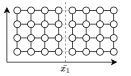
\includegraphics[width=\textwidth]{images/coord_1.drawio.svg.pdf}
        \caption{}
        \label{fig:coord_1}
    \end{subfigure}
    \hfill
    \begin{subfigure}[b]{0.23\textwidth}
        \centering
        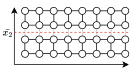
\includegraphics[width=\textwidth]{images/coord_2.drawio.svg.pdf}
        \caption{}
        \label{fig:coord_2}
    \end{subfigure}
    \caption{Bisection of the graph along the $x_1$-axis, resulting in a 4-edge cut (left),
    and along the $x_2$-axis, resulting in 8-edge cut (right). The $x_1$-axis bisection is selected.}
    \label{fig:coord}
\end{figure}
    \begin{algorithm}
    \caption{Coordinate bisection.}
    \label{alg:coord}
    \begin{algorithmic}[1]
        \Require Graph \( G = (\mathcal{V}, \mathcal{E}) \), points \( P_i = (x_{1}, \dots, x_{d})_i \)
        \Ensure A bisection of \( G \) into \(\mathcal{V}_1\) and \(\mathcal{V}_2\)
        \Function{coordinate\_part}{graph $G$, points $P_i$}
            \State Initialize $c_{\min} \gets \infty$, $j^* \gets 1$
            \For{each axis \( x_j \), \( j = 1, \dots, d \)}
                \State Compute the median \(\bar{x}_j\)
                \State Compute the edge cut \( c_j \) for the bisection at \(\bar{x}_j\)
                \If{ \( c_j < c_{\min} \) }
                    \State $c_{\min} \gets c_j$
                    \State $j^* \gets j$
                \EndIf
            \EndFor
            \State Partition \(\mathcal{V}\) into \(\mathcal{V}_1\) and \(\mathcal{V}_2\) via \(\bar{x}_{j^*}\) bisection
            \State \Return \(\mathcal{V}_1, \mathcal{V}_2\)
        \EndFunction
    \end{algorithmic}
\end{algorithm}
    
    The coordinate bisection method in \texttt{GraphLab.jl} can be invoked using the following command:
    
    \begin{lstlisting}[language=Julia]
    GraphLab.part_coordinate(A, coords)
    \end{lstlisting}
    
    The coordinate bisection algorithm is computationally efficient and conceptually simple.
    However, its effectiveness is strongly influenced by the choice of coordinate system.
    A mere rotation of the coordinate axes can lead to significantly different partitioning results,
    as the algorithm strictly aligns the division with the coordinate axes.
    This sensitivity may lead to suboptimal partitions, particularly in cases where the problem geometry
    is not naturally aligned with the axes, highlighting a fundamental limitation of the algorithm in certain applications.
%%%%%%%%%%%%%%%%%%%%%%%%%%%%%%%%%%%%%%%%%%%%%%%%%%%%%%%%%%%%%%   
    \subsubsection{Inertial bisection}
    The inertial bisection mitigates the axis-alignment limitation of coordinate bisection by
    allowing the dividing hyperplane to be orthogonal to a direction determined by the
    distribution of vertices rather than a fixed coordinate axis. This approach ensures that
    partitioning is guided by the intrinsic geometry of the data rather than an arbitrary reference frame.
    In two dimensions, the dividing hyperplane is
    represented by a line $l$ that minimizes the sum
    of squared distances from the vertices to the line. The algorithm first determines the center of mass of the vertex set,
    \begin{equation}
      \bar{P}=(\bar{x}, \bar{y}), \quad \text{where} \quad  \bar{x} = \frac{1}{n}\sum_{i=1}^n x_i, \quad \bar{y} = \frac{1}{n}\sum_{i=1}^n y_i\text{.}
    \end{equation}
    It then defines a unit direction vector $\mathbf{u}=[u_1, u_2]^T$, such that 
    $\|\mathbf{u}\|_2 = \sqrt{u_1^2+u_2^2} = 1$.
    The parametric equation
    of the bisecting line is given by
    $l(\lambda) = \{\bar{P} + \lambda \mathbf{u}  \mid \lambda \in \mathbb{R} \}$.
    
    \begin{figure}[h!]
    \centering
    \begin{subfigure}[b]{0.23\textwidth}
        \centering
        \includegraphics[width=\textwidth]{images/inert_0.drawio.svg.pdf}
        % \caption{}
        \label{fig:inert_1}
    \end{subfigure}
    \hfill
    \begin{subfigure}[b]{0.23\textwidth}
        \centering
        \includegraphics[width=\textwidth]{images/inert.drawio.svg.pdf}
        % \caption{}
        \label{fig:inert_2}
    \end{subfigure}
    \caption{Illustration of the inertial bisection in 2D: dividing the graph
    along the line orthogonal to the direction $\mathbf{u}$ through the center of mass $\bar{P}$ that minimizes the sum of squared distances.}
    \label{fig:inert}
\end{figure}
    
    % The coordinates of the center of mass $\bar{P}$, which lies on the line $l$, are given by
    
    
    To determine the optimal orientation of the bisecting hyperplane, the unit direction vector $\mathbf{u}$ is chosen to minimize the sum of the squared
    distances from the vertices to the line:
    
    \begin{equation} 
\begin{aligned}[b]
    \sum_{i=1}^n d_i^2 
    &= \sum_{i=1}^n(x_i - \bar{x})^2+(y_i - \bar{y})^2\\
    &-(u_1(x_i - \bar{x})+u_2(y_i - \bar{y}))^2 \\
    &=(1-u_1^2)\sum_{i=1}^n(x_i - \bar{x})^2+
    (1-u_2^2)\sum_{i=1}^n(y_i - \bar{y})^2\\
    &+2u_1u_2\sum_{i=1}^n(x_i - \bar{x})(y_i - \bar{y})\\
    &= (1-u_1^2)S_{xx}+
    (1-u_2^2)S_{yy}+2u_1u_2S_{xy}\\
    &=\mathbf{u}^T
    \vcenter{
        \hbox{$
        \begin{pmatrix}
        S_{xx} & S_{xy} \\
        S_{xy} & S_{yy}
        \end{pmatrix}
        $}
    } \label{eq:projection_matrix}
    \mathbf{u} = \mathbf{u}^T\mathbf{M}\mathbf{u}
\end{aligned}
\end{equation}
    
    Here, $\mathbf{M}$ is a symmetric matrix, and its smallest eigenvalue corresponds to the minimal sum of the squared distances. Consequently, the optimal direction vector $\mathbf{u}$ is given by the
    normalized eigenvector associated with the smallest eigenvalue of
    $\mathbf{M}$ \cite{elsner1997graph}. This choice ensures that the partitioning hyperplane is aligned with the principal axis of least variance, making the algorithm robust to coordinate system transformations. The full procedure for bisecting a graph using inertial partitioning is summarized in \Cref{alg:inert}.
    
    \begin{algorithm}
    \caption{Inertial bisection.}
    \label{alg:inert}
    \begin{algorithmic}[1]
        \Require Graph \( G = (\mathcal{V}, \mathcal{E}) \), points \( P_i = (x_{1}, \dots, x_{d})_i \)
    \Ensure A bisection of \( G \) into \(\mathcal{V}_1\) and \(\mathcal{V}_2\)
    \Function{inertial\_part}{graph $G$, points $P_i$}
        \State Calculate the center of mass $\bar{P}$
        \State Compute eigenvec. associated with smallest eigenval. of $\mathbf{M}$
        \State Partition the vertices $\mathcal{V}$ around the line $l$
        \State \Return \(\mathcal{V}_1, \mathcal{V}_2\)
    \EndFunction
    \end{algorithmic}
\end{algorithm}

    To perform inertial bisection with \texttt{GraphLab.jl} on a graph, use:

    \begin{lstlisting}[language=Julia]
    GraphLab.part_inertial(A, coords)
    \end{lstlisting}

%%%%%%%%%%%%%%%%%%%%%%%%%%%%%%%%%%%%%%%%%%%%%%%%%%%%%%%%%%%%%%
    \subsubsection{Random sphere bisection}
    \label{sub:rand_sphere}
    The random sphere method \cite{doi:10.1137/S1064827594275339} partitions a graph
    by exploiting spatial information to identify separators that align with the intrinsic geometry of the vertex
    distribution.
    Instead of relying on axis-aligned or moment-based directions,
    this approach uses randomized geometric projections to discover low-cut partitions.
    The algorithm initially normalizes the vertex by translating and scaling the vertex coordinates to ensure the distribution is centered at the origin and confined within a unit-scale region.
    It subsequently maps the vertex coordinates onto the unit sphere via stereographic projection, thereby embedding the original Euclidean geometry into a higher-dimensional spherical manifold.

    To identify effective separators, the algorithm selects
    several approximate center points on the sphere, each obtained as the coordinate-wise median of a randomly sampled subset of vertices.
    Around each center point, a conformal transformation is applied to recenter the spherical embedding, thereby increasing the likelihood that sampled circles align with meaningful structures in the graph.
    For each transformed configuration, the algorithm samples
    multiple directions on the sphere, each defining a candidate circle separator.
    Vertices are then partitioned according to the sign of their
    inner product with the chosen direction vector, effectively
    dividing the sphere into two hemispheres.

    In addition to spherical separators, the method also considers a set of random linear cuts in the original
    Euclidean space. Each linear cut is defined by a hyperplane
    orthogonal to a randomly sampled direction and positioned to
    bisect the vertex set at the median projection values.
    The final output is the spherical or linear partition that minimizes the total edge cut.

    The random spherical bisection algorithm implemented in \texttt{GraphLab.jl} is described in \Cref{alg:sphere} and can be applied with:

    \begin{lstlisting}[language=Julia]
    GraphLab.part_randsphere(A, coords; ntrials)
    \end{lstlisting}

    An optional argument \texttt{ntrials} specifies the number of random directions to try.

    \begin{algorithm}
    \caption{Random sphere bisection.}
    \label{alg:sphere}
    \begin{algorithmic}[1]
        \Require Graph \( G = (\mathcal{V}, \mathcal{E}) \), points \( P_i = (x_{1}, \dots, x_{d})_i \)
    \Ensure A bisection of \( G \) into \(\mathcal{V}_1\) and \(\mathcal{V}_2\)
    \Function{random\_sphere\_part}{graph $G$, points $P_i$}
        \State Calculate the center of mass \(\bar{P}\)
        \State Normalize \(P_i \rightarrow \tilde{P_i} = (P_i - \bar{P})/\max_j{|P_j - \bar{P}|}\)
        \State Project each \(\tilde{P_i}\) onto the unit sphere \(\tilde{P_i}\rightarrow Z_i \in \mathcal{S}^d\)
        \For{each of \( s \) random center points}
            \State Select a random subset of points from \(Z\)
            \State Compute coordinate-wise median \(c\)
            \State Apply conformal map to move \(c\) to the origin
            \For{each random directions \(u\)}
                \State \(\mathcal{V}_1 \gets { i \mid \langle Z_i, u \rangle \leq 0 }, \quad \mathcal{V}_2 \gets { i \mid \langle Z_i, u \rangle > 0 } \)
                \State Select \(\mathcal{V}_1\), \(\mathcal{V}_2\) with the smallest edge cut
            \EndFor
        \EndFor
        \State \Return \(\mathcal{V}_1\), \(\mathcal{V}_2\)
    \EndFunction
    \end{algorithmic}
\end{algorithm}
    
%%%%%%%%%%%%%%%%%%%%%%%%%%%%%%%%%%%%%%%%%%%%%%%%%%%%%%%%%%%%%%   
    \subsubsection{Adaptive space-filling curves}
    \label{sub:sfc}
    Space-filling curves (SFCs) provide a continuous, one-dimensional traversal
    of multidimensional space that preserves spatial locality.
    In the context of partitioning, SFCs induce a linear ordering of the data
    points, enabling recursive division into balanced and spatially coherent subregions. In this work, we implement an adaptive SFC traversal over a
    hierarchical spatial decomposition to generate partitions that reflect the geometric structure of the input graph \cite{Sasidharan15, sasidharan2015space}.

    The algorithm, presented in \Cref{alg:adaptive_sfc}, performs coordinate bisection as introduced in \Cref{subsubsec:coord} based on spatial distribution of the graph's vertices, using an adaptive SFC traversal.
    It begins by constructing a KD-tree of the vertex coordinates $P$, where, at each node, the splitting axis is chosen according to the direction of maximum spatial extent. The point set $P$ is then recursively divided until each leaf contains a single point.

    Once the tree is built a, an adaptive SFC traversal defines a linear order of the leaves by visiting spatial regions in a directionally consistent, locality-preserving manner. This process is governed by entry and exit directions propagated recursively. The coordinates associated with each leaf are collected in the order of traversal, yielding a one-dimensional sequence.
    This process is illustrated in \Cref{fig:sfc}.

    The resulting sequence is subsequently partitioned into $k$ contiguous segments of approximately equal size, producing $k$ spatially coherent and locality-preserving partitions. A key advantage of this method over other partitioning approaches is that, once the traversal is computed, partitioning into an arbitrary number of parts becomes a trivial post-processing step: splitting the ordered node list into contiguous segments.

    Adaptive space-filling curve partitioning in \texttt{GraphLab.jl} is invoked as follows, with an optional argument \texttt{k} specifying the number of partitions:
    
    \begin{lstlisting}[language=Julia]
    GraphLab.part_adaptive_sfc(A, coords, k)
    \end{lstlisting}

    \begin{figure}
\centering

% Left column: two stacked figures
\begin{minipage}{0.29\textwidth}
    \begin{subfigure}{\textwidth}
        \centering
        \includegraphics[width=\textwidth]{images/sfc_adaptive.svg.pdf}
        \caption{}
        \label{fig:sfc_adaptive}
    \end{subfigure}

    % \vspace{0.5cm} % Adjust spacing as needed

    \begin{subfigure}{\textwidth}
        \centering
        \includegraphics[width=\textwidth]{images/sfc_kdtree.svg.pdf}
        \caption{}
        \label{fig:sfc_kdtree}
    \end{subfigure}
\end{minipage}
\hfill
% Right column: one tall figure
\begin{minipage}{0.13\textwidth}
    \begin{subfigure}[b]{\textwidth}
        \centering
        \includegraphics[width=\textwidth]{images/sfc_traversal.svg.pdf}
        \caption{}
        \label{fig:sfc_traversal}
    \end{subfigure}
\end{minipage}

\caption{The adaptive space-filling curve (SFC) partitioning process begins with the recursive spatial subdivision of the input domain (a), followed by the construction of the corresponding KD-tree (b). Then, a direction-aware recursive traversal defines a linear ordering of the leaf nodes (c). In this example, the resulting order is $v_3 \rightarrow v_2 \rightarrow v_4 \rightarrow v_5 \rightarrow v_7 \rightarrow v_8 \rightarrow v_6 \rightarrow v_1$.}
\label{fig:sfc}
\end{figure}
    
    \begin{algorithm}
    \caption{Adaptive Space-Filling Curve Partitioning.}
    \label{alg:adaptive_sfc}
    \begin{algorithmic}[1]
        \Require Graph \( G = (\mathcal{V}, \mathcal{E}) \), points \( P_i = (x_{1}, x_{2})_i \), number of parts \(k\)
        \Ensure A partition of \( G \) into \( k \) parts
        \Function{adaptive\_sfc\_partition}{graph $G$, points $P_i$, $k$}
            \State Build spatial tree \(T \gets\) \Call{build\_tree}{$P_i$}
            \State Traverse \(T\): \(order \gets\) \Call{traverse\_sfc}{$T$, $L$, $R$}
            \State Partition the linear \(order\) into \(k\) balanced parts
            \State \Return the \(k\) partitions of \(\mathcal{V}\)
        \EndFunction
        \Function{build\_tree}{points $P_i$}
            \If{\(|P_i| = 1\)}
                \State \Return leaf node containing \(P_1\)
            \Else
                \State Compute bounding box of \(P_i\)
                \State Divide \(P_i\) into two subsets \(P^-\), \(P^+\)
                \State Node \(N_{\text{left}} \gets\) \Call{build\_tree}{$P^-$}
                \State Node \(N_{\text{right}} \gets\) \Call{build\_tree}{$P^+$}
                \State \Return node with \(N_{\text{left}}\) and \(N_{\text{right}}\) as children
            \EndIf
        \EndFunction
        \Function{traverse\_sfc}{node $N$, entry, exit, accumulator $a$}
            \If{\(N\) is a leaf}
                \State exit \(\gets\) coord. of \(N\)
                \State Append \(N\) to \(a\)
                \State \Return exit
            \Else
                \State Determine child order based on SFC rules
                \For{each child in order}
                    \State Recursively traverse child with updated entry/exit
                \EndFor
                \State \Return \(a\)
            \EndIf
        \EndFunction
    \end{algorithmic}
\end{algorithm}
    

%%%%%%%%%%%%%%%%%%%%%%%%%%%%%%%%%%%%%%%%%%%%%%%%%%%%%%%%%%%%%%
% Non-geometric-based
%%%%%%%%%%%%%%%%%%%%%%%%%%%%%%%%%%%%%%%%%%%%%%%%%%%%%%%%%%%%%%
    \subsection{Non-geometric-based partitioning algorithms}
    \label{subsec:non-geo}
    Geometric-based partitioning algorithms are efficient techniques for partitioning meshes, particularly
    when spatial adjacency plays a key role in connectivity. However, these algorithms have inherent limitations.
    They rely on the assumption that the graph's vertices exhibit a spatial relationship, an assumption that does not
    hold in all contexts, such as social networks\cite{Newman_2013} or parallel processing\cite{10.1145/2503210.2503293}.
    
    To accommodate a broader range of applications, alternative algorithms that do not rely on geometric information
    have been developed. Notable examples include the Kernighan-Lin algorithm\cite{6771089} and graph-growing algorithms\cite{doi:10.1137/S1064827595287997},
    both well suited for partitioning graphs an lacking explicit spatial structure.
    Among these, spectral bisection is a particularly powerful technique, leveraging
    the eigenvalues and eigenvectors of the graph Laplacian matrix to inform partitioning decision\cite{fiedler75}.
    In this subsection, we focus
    on the implementation and application of spectral bisection, detailing its computational properties and advantages over geometry-dependent algorithms.
%%%%%%%%%%%%%%%%%%%%%%%%%%%%%%%%%%%%%%%%%%%%%%%%%%%%%%%%%%%%%%    
    \subsubsection{Spectral bisection}\label{sub:spec} The spectral bisection algorithm partitions a graph
    by leveraging the eigenvector corresponding to the second-smallest eigenvalue
    --- commonly known as the Fiedler vector--- of the graph's Laplacian matrix $\mathbf{L}$.
    The Laplacian matrix is defined as:
    \begin{equation}
        \mathbf{L} = \mathbf{D}-\mathbf{A},
    \end{equation}
    where $\mathbf{D}$ is the degree matrix and $\mathbf{A}$ is the adjacency matrix.
    The graph Laplacian $\mathbf{L}$ is a symmetric, positive semi-definite matrix, ensuring the existence of an orthogonal basis of eigenvectors $\mathbf{u}^{(i)}$ with corresponding eigenvalues
    $\lambda^{(i)}$.
    The smallest eigenvalue, $\lambda^{(1)} = 0$, and its associated eigenvector
    $\mathbf{u}^{(1)} = c\mathbf{1}$, where $c$ is a constant and $\mathbf{1}$ is the all one’s vector, correspond to the trivial solution that reflects the connectivity of
    the entire graph.
    The eigenvector $\mathbf{u}^{(2)}$
    associated with the second-smallest eigenvalue $\lambda^{(2)}$, known as the Fiedler vector\cite{fiedler75}, captures intrinsic connectivity pattern of the graph, as illustrated in \Cref{fig:spec}.
    
    Each node $v_i$ is associated with the corresponding entry $\mathbf{u}^{(2)}_i$ of the Fiedler vector. The partition is performed by thresholding these values:
    \begin{itemize}
        \item A threshold at zero yields two roughly balanced subsets while minimizing the edge cut.
        \item A threshold at $\mathbf{u}^{(2)}$ results in two strictly equal-sized partitions.
    \end{itemize}
    The complete spectral bisection algorithm is outlined in \Cref{alg:spec}, detailing its key computational steps.
    
    \begin{figure}[h!]
    \centering
    \begin{subfigure}[b]{0.20\textwidth}
        \centering
        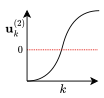
\includegraphics[width=\textwidth]{images/spec_u.svg.pdf}
        % \caption{}
        \label{fig:spec_1}
    \end{subfigure}
    \hfill
    \begin{subfigure}[b]{0.23\textwidth}
        \centering
        \includegraphics[width=\textwidth]{images/spec_g.drawio.svg.pdf}
        % \caption{}
        \label{fig:spec_2}
    \end{subfigure}
    \caption{Plot of the values of $\mathbf{u}^{(2)}$, where each $\mathbf{u}^{(2)}_i$ corresponds to vertex
    $v_i$ in the original sequence, and where $\mathbf{u}^{(2)}_k$ corresponds to $v_k$ in the reordered sequence, such that $\mathbf{u}^{(2)}_1 < \mathbf{u}^{(2)}_2 < \dots < \mathbf{u}^{(2)}_n$ (left).
    The graph partitions corresponding to this ordering (right), with the threshold $\epsilon = 0$ defining the cut (right).
    }
    \label{fig:spec}
\end{figure}
    
    \begin{algorithm}
    \caption{Spectral bisection.}
    \label{alg:spec}
    \begin{algorithmic}[1]
        \Require Graph \( G = (\mathcal{V}, \mathcal{E}) \)
    \Ensure A bisection of \( G \) into \(\mathcal{V}_1\) and \(\mathcal{V}_2\)
    \Function{spectral\_part}{graph $G$}
        \State Form the Laplacian matrix \(\mathbf{L}\)
        \State Compute the 2nd smallest eigenval. \(\lambda^{(2)}\) and eigenvec. \(\mathbf{u}^{(2)}\)
        \State Set 0 or the median of \(\mathbf{u}^{(2)}\) as threshold \(\epsilon\)
        \State Set \(\mathcal{V}_1 := \{v_i \in \mathcal{V} \mid u_i< \epsilon\}\), \(\mathcal{V}_2 := \{v_i \in \mathcal{V} \mid u_i \geq \epsilon\}\)
        \State \Return \(\mathcal{V}_1, \mathcal{V}_2\)
    \EndFunction
    \end{algorithmic}
\end{algorithm}

    Spectral bisection method implemented in \texttt{GraphLab.jl} can be executed with:

    \begin{lstlisting}[language=Julia]
    GraphLab.part_spectral(A)
    \end{lstlisting}

    It requires only the adjacency matrix \texttt{A} as input and returns a vector assigning each node to partition 1 or 2.


%%%%%%%%%%%%%%%%%%%%%%%%%%%%%%%%%%%%%%%%%%%%%%%%%%%%%%%%%%%%%%
% Hybrid bisection
%%%%%%%%%%%%%%%%%%%%%%%%%%%%%%%%%%%%%%%%%%%%%%%%%%%%%%%%%%%%%%
    \subsection{Hybrid partitioning algorithms}
    \label{subsec:hybrid}
    Building on the random sphere bisection and the spectral partitioning described in \ref{sub:rand_sphere} and \ref{sub:spec}, hybrid bisection extends spectral methods with
    a randomized geometric layer to enhance partitioning quality, particularly in graphs with an underlying spatial structure.

    The method begins by computing a spectral embedding of the graph, in which each vertex is mapped to a point in $\mathbb{R}^d$ using the first $d$ nontrivial eigenvectors of the Laplacian matrix. This embedding encodes the global
    connectivity structure of the graph in a continuous geometric space, often revealing natural separations aligned
    with sparse cuts.

    The embedded point cloud is partitioned with the random sphere method. This process effectively performs a geometric search over separators, guided by the spectral structure of the graph.

    The hybrid method leverages the algebraic properties of spectral embeddings alongside the geometric adaptability of random sphere cuts to generate balances and spatially localized partitions.

    Geometric spectral partitioning in \texttt{GraphLab.jl} can be executed with:

    \begin{lstlisting}[language=Julia]
    GraphLab.part_geospectral(A; ev=d)
    \end{lstlisting}

    In addition to the adjacency matrix \texttt{A}, it optionally accepts $\texttt{ev}=d$ the number of nontrivial Laplacian eigenvectors to use for embedding (default: 2).
    
%%%%%%%%%%%%%%%%%%%%%%%%%%%%%%%%%%%%%%%%%%%%%%%%%%%%%%%%%%%%%%
% Recursive bisection
%%%%%%%%%%%%%%%%%%%%%%%%%%%%%%%%%%%%%%%%%%%%%%%%%%%%%%%%%%%%%%
    \subsection{Recursive bisection and nested dissection}
    Recursive bisection and nested dissection are techniques that rely on recursively partitioning a graph into smaller subgraphs. While recursive bisection is primarily used to generate multiple balanced partitions, nested dissection applies a recursive strategy to reduce fill-in during sparse matrix factorization. This section outlines both methods and their respective algorithmic formulations.
    \subsubsection{Recursive bisection}
    \label{subsub:rec_bi}
    A straightforward and effective strategy for partitioning a graph into $p = 2^q$ parts,
    where $q$ is a positive integer, is recursive bisection, as presented in \Cref{alg:recursive}.
    This algorithm iteratively applies graph bisection, progressively
    subdividing the graph into smaller sub-graphs.
    In \texttt{GraphLab.jl}, recursive bisection can be used with any of the bisection algorithms presented in \Cref{subsec:geo,subsec:non-geo}.
    The algorithm is built around a recursive function, \texttt{Recursion}, which takes as inputs:
    \begin{itemize}
        \item $C'$, the current sub-graph to be partitioned,
        \item $p'$, the number of partitions into which $C'$ will be further divided, and
        \item $\mathrm{idx}$, an integer tracking the position of the first part of $C'$ in the final partitioning results.
    \end{itemize}
    
    At each recursive step, the sub-graph $C'$ is bisected into two balanced parts. The process continues
    until the desired number of partitions, $p = 2^q$, is obtained. This recursive strategy results in a structured,
    hierarchical decomposition of the graph, making it particularly well suited for parallel computing applications, especially in domains like finite element and finite difference methods\cite{doi:10.1137/S1064827593255135}. 
    
    \begin{algorithm}
    \caption{Recursive bisection.}
    \label{alg:recursive}
    \begin{algorithmic}[1]
        \Require Graph \( G = (\mathcal{V}, \mathcal{E}) \)
    \Ensure A $p$-way partition of \( G \)
    \State \(G_p = \{C_1,\dots, C_p\}\)
    \State \(p = 2^l\)
    \Function{rec\_bisection}{graph $G$, number of parts $p$}
        \Function{recursion}{$C'$, $p'$, $\mathrm{idx}$}
            \If{\(p'\) \text{is even}}
                \State \(p' \leftarrow \frac{p'}{2}\)
                \State \(\left(C'_1, C'_2\right)\leftarrow \)\Call{bisection}{$C'$}
                \State \Call{recursion}{$C'_1$, $p'$, $\mathrm{idx}$}
                \State \Call{recursion}{$C'_2$, $p'$, $\mathrm{idx}+p'$}
            \Else
                \State \(C_{\mathrm{idx}} \leftarrow C'\)
            \EndIf
        \EndFunction
         \State \Call{recursion}{$C$, $p$, $1$}
         \State \Return \(G_p\)
    \EndFunction
    \end{algorithmic}
\end{algorithm}

    \texttt{GraphLab.jl} provides a recursive interface for all partitioning algorithms described in \Cref{sec:algo}, which can be invoked with:

    \begin{lstlisting}[language=Julia]
    GraphLab.recursive_bisection(method, k, 
        A, coords)
    \end{lstlisting}

    Here, \texttt{method} is any partitioning function available in the package, \texttt{k} is the desired number of partitions (if not a power of two, it is automatically rounded up to the nearest power of two), and \texttt{A} and \texttt{coords} are the graph's adjacency matrix and node coordinates. The function returns a vector assigning each node a label from 1 to \texttt{k}, indicating its partition membership.


    \subsubsection{Nested dissection}
    The nested dissection ordering algorithm is a multilevel heuristic introduced to minimize fill-in, i.e., the creation of nonzero entries during sparse matrix factorizations\cite{George73}.
    It recursively partitions a graph $G$ through the identification of balanced vertex separators, which are removed to decompose $G$ into disconnected components. The same procedure is then applied recursively to each subgraph.
    Unlike standard recursive bisection, as described in \Cref{subsub:rec_bi}, which directly bisects the graph into two parts, nested dissection introduces an intermediate step: the explicit computation of a separator whose removal divides the problem into independent subproblems.
    To compute the separator, border vertices are first identified between the two subdomains resulting from the initial bisection. These vertices induce a bipartite graph, where edges represent adjacency across the partition boundary. A maximum matching is then computed on this bipartite graph; this matching corresponds to a minimum vertex cover\cite{turner2020mappingmatchingsminimumvertex, storer2012introduction}, providing an efficient approximation of a small separator. The selected separator vertices are removed, and the nested dissection proceeds recursively on the resulting components.
    The final ordering $\pi$ places all separator vertices after the recursively ordered interior vertices, yielding a global vertex ordering that preserves sparsity patterns. The overall process is outlined in \Cref{alg:nested_dis}.

    This strategy is widely used in the symbolic factorization phase of sparse direct solvers, where it facilitates the construction of efficient elimination trees and reduces both fill-in and memory overhead during numerical factorization.
    Nested dissection can be implemented using partitioning methods presented in \Cref{subsec:geo} and \Cref{subsec:non-geo} for separator computation, making it a flexible tool in both partitioning and numerical linear algebra contexts.

    \begin{algorithm}
    \caption{Nested dissection ordering.}
    \label{alg:nested_dis}
    \begin{algorithmic}[1]
        \Require Adj. matrix \( A \), partitioning \textsc{method}, minimum separator size $\mathrm{minsep}$
        \Ensure Permutation vector \(\pi\) s.t. \(A[\pi, \pi]\) has reduced fill-in
        \Function{nested\_dis}{$A$, \textsc{method}, $\mathrm{coords}$ (opt.), $\mathrm{minsep}$}
            \State Identitfy connected components of \(A\)
            \State Initialize permutation vector \(\pi\)

            \For{each component \(C\)}
                \If{\(|C| \leq \mathrm{minsep}\)}
                    \State Apply minimum degree ordering on \(A[C, C]\)
                \Else
                    \State Bisect \(C \rightarrow C_1, C_2\) via \textsc{method} 
                    \State Identify separator nodes between \(C_1\) and \(C_2\)
                    \State Recursively compute orderings:
                    \State \hspace{2em}$\pi_1 \gets$ \Call{nested\_dis}{$A[C_1, C_1]$}
                    \State \hspace{2em}$\pi_2 \gets$ \Call{nested\_dis}{$A[C_2, C_2]$}
                    \State Combine \(\pi_C \gets [\pi_1, \pi_2, \text{separator}]\)
                \EndIf
                \State Insert \(\pi_C\) into global permutation \(\pi\)
            \EndFor
            
            \State \Return \(\pi\)
        \EndFunction
    \end{algorithmic}
\end{algorithm}

    The nested dissection provided by \texttt{GraphLab.jl} can be called using:

    \begin{lstlisting}[language=Julia]
    GraphLab.nested_dissection(A, method; 
        coords, minsep=5)
    \end{lstlisting}

    The inputs are the adjacency matrix \texttt{A}, any partitioning \texttt{method} from \texttt{GraphLab.jl}, and the node coordinates \texttt{coords} if required by the chosen method. An optional argument \texttt{minsep} specifies the minimum separator size (default: 5). The output is a permutation vector representing the nested dissection ordering.
    
\end{document}